% Sample file for AES paper
\documentclass[fleqn]{jaes}

% Metadata Information
\jyear{2026}
\jmonth{April}
%\jvol{69}
%\jnum{3}
\jname{Universidad Nacional de San Agustín de Arequipa}
\usepackage{amsmath}\setlength{\mathindent}{10pt}
\usepackage{bm}
\usepackage[capitalise]{cleveref}
  \crefformat{section}{\textsc{Sec.~#2#1#3}}
  \Crefformat{section}{\textsc{Sec.~#2#1#3}}
  \crefformat{figure}{{Fig.~#2#1#3}}
  \Crefformat{figure}{{Fig.~#2#1#3}}
  \crefformat{table}{{Table~#2#1#3}}
  \Crefformat{table}{{Table~#2#1#3}}

%% Template speific, to remove
% \usepackage{draftwatermark}
% \SetWatermarkText{RUSSELL}
% \SetWatermarkColor[gray]{0.9}
% \SetWatermarkScale{0.85}

% \usepackage[left]{lineno} % [switch] option for outside two-column not compatibal with JAES template
% \linenumbers

%\usepackage{citesort}

% Tested successfully with todonotes pkg
% \usepackage[]{todonotes}
% \newcommand{\mytodo}[1]{\todo[inline,color=blue!10]{Todo: #1}}

\begin{document}

% Page heads {Authors}{Short title}
% \markboth{DUPONT AND DOE}{JAES TEMPLATE 2026}

% Title portion
\title{Visual Analytics de Representaciones Aprendidas en la Fusión Multimodal de Señales EEG y Fisiológicas: un Caso de Estudio sobre DEAP}

%Author Info.
% \authorgroup{
% \author{JEAN DUPONT,\textsuperscript{1}\orcidlink{0000-0001-2345-6789}\thanks{To whom correspondence should be addressed, email: journal.editorinchief@aes.org.}}
% \aesrole{Member}{70748}, % For AES members, provide current membership role (Member, Associate Member, Student Member, or Life Member) and AES membership number
% AND \author{JANE DOE,\textsuperscript{2}}
% \aesrole{Fellow}{43549} 
% \email{(jean.dupont@xyz.edu)\quad\quad\quad\quad\quad\quad\quad\quad\quad\quad\quad (jane\_doe@company.com)}
% \affil{\textsuperscript{1}Acoustic Research Laboratory, Department of Sound Processing, XYZ University, City, Country \\
% \textsuperscript{2}Audio Technology Company, City, State, USA}
% }
\authorgroup{
\author{Jorge Tito Ccahuaya\textsuperscript{1}}
\email{jtitoc@unsa.edu.pe}
\affil{\textsuperscript{1}Escuela Profesional de Ciencia de la Computación, Universidad Nacional de San Agustín de Arequipa, Arequipa, Perú}
}

%Abstract
\abstract{%
% An informative and self-contained abstract of 100 to 200~words must be provided. The abstract should mention the motivation, problem statement, approach, results, and implications of the work, usually with one or two sentences each. The abstract should be written in a single paragraph without citing any references. The \textit{Journal of the Audio Engineering Society} is a modern scientific journal supporting online publishing with colors and a graphical abstract. It is a hybrid access journal publishing both Open Access and traditional papers, the latter being available for subscribers, such as AES members, or at an individual article access fee. If a paper published in the \textit{Journal of the Audio Engineering Society} has been made Open Access, it will have the OA logo next to it and will be freely downloadable from the AES E-Library by anyone, even if they are not an AES member or E-Library subscriber. This example abstract contains 151~wordss.
TODO
}
\maketitle

% Keywords, provide approximately 3 keywords
\begin{keywords}
Affective computing, EXG, Multimodal fusion, Visual analytics
\end{keywords}

%Head 1
\section{Introduction}
The \emph{Journal of the Audio Engineering Society (JAES)} seeks original unpublished Research Papers and Engineering Reports of archive quality on subjects related to the audio domain. All submissions will go through a peer-review process to check their suitability for \emph{JAES}. Manuscripts should describe original work unpublished elsewhere or not being considered for publication elsewhere. The different types of possible submission are
\begin{itemize}
    \item Research Paper,
    \item Engineering Report,
    \item Review/Tutorial Paper, 
    \item Communication, and
    \item Letter to the Editor.
\end{itemize}

Full details of these submission types are given on the AES Journal Manuscript Types description page.\footnote{\url{https://aes2.org/publications/journal-of-the-audio-engineering-society/aes-journal-manuscript-types/}} All articles accepted for publication exceeding ten (10) pages will be subject to page fee charges. Please always refer to the  Author Guidelines web page to be sure that you follow the latest rules.\footnote{\url{https://aes2.org/publications/journal-of-the-audio-engineering-society/journal-author-guidelines/}.}

Authors should submit a manuscript for review to the online submission and peer-review system.\footnote{\url{https://aes2.org/publications/journal-of-the-audio-engineering-society/submit-a-paper-to-the-aes-journal/}.} Manuscripts are reviewed anonymously by members of the review board, invited from the scientific and industry-led community. 
Prior to being sent for review, the manuscript is checked for relevance to the journal. Authors should check the list of topics treated by the journal\footnote{\url{https://aes2.org/publications/journal-of-the-audio-engineering-society/aes-journal-indicative-topic-list/}.} and indicate the appropriate category on submission. One general check for relevance to the journal is whether or not prior articles in the \emph{JAES} are cited. If this is not the case, or a suitable category is not listed, the authors should provide a clear argument for consideration by the journal to the Editor upon submission. In absence of such justification, or if considered not appropriate to the journal, the manuscript will likely receive a \emph{desk reject} decision. 
After the reviewers’ analysis and recommendation to the editors, the author is promptly advised of the decision. On the basis of the reviewers’ comments, the Editor may request that the author make certain revisions that could allow the paper to be accepted for publication.

A growing number of \emph{JAES} papers are published as Open Access articles. They are freely available to read for all, not only to AES Members. This is certain to attract more readers and citations for these articles. The authors of each paper can decide whether they want their work to be available like this. The AES policy on Open Access is explained in detail on the Open Access web pages: \url{https://aes2.org/publications/open-access-publications-policy/}.

The final paragraph of the Introduction should briefly summarize the contents of the rest of the paper. \Cref{sec:org} describes how the paper may be organized and how equations, figures, tables, and a graphical abstract are formatted. The reference format is described in \cref{sec:refs}. \Cref{sec:authophoto} gives instructions about author photographs and biographies. \Cref{sec:AI-LLM} provides guidance on the acceptable appropriate use and citation for artificial intelligence (AI)/large language models (LLMs) in the journal. \Cref{sec:general} lists the basic requirements for \emph{JAES} papers, and \cref{sec:conc} concludes. 

\section{Organization}{\label{sec:org}}

Technical articles published in \emph{JAES} should be informative and well organized. They should cite original work or review previous work, giving proper credit. Results of actual experiments or research should be included. The journal cannot accept unsubstantiated or commercial statements. Authors should observe the general requirements for AES publications, as agreed by the Publications Policy Committee, given in \cref{sec:general} of this template.

The paper title should be short, accurate, and interesting. It should give an idea of the type of work. For example, the title of a Research Paper should highlight the main application or advantage of the presented work. Similarly, a Review/Tutorial article should have a broad and inclusive title. The paper title should include the essential keyword(s) to attract readers. The words “new” and “novel” in the paper title are prohibited. Repeating a word in the title is not recommended.
The use of domain-specific acronyms or uncommon words in the title is discouraged because they limit the number of potential readers, while they can be included among the keywords. A list of approved acronyms for use in titles is provided in \textsc{Appendix}~\ref{sec:ackronyms}. Article short titles must be about 60~characters, including spaces.

Three to five keywords describing the field and contents of the article should be inserted in alphabetical order below the Abstract. Keywords should give additional information beyond the paper title. Please choose commonly used keywords to describe the field of work and the methods used, such as those appearing in the IEEE Taxonomy list \cite{ieee-taxonomy}. Please do not invent new terms, as they are not helpful for classification or searching. Do not repeat consecutive words from the article title as keywords, but use synonyms instead. 

The manuscript should develop the main point, beginning with a section entitled ``Introduction'' and ending with a ``Conclusion''. Subheads are appropriate and should be inserted where necessary. Section division numbers should be of the form 1, 1.1, 1.1.1, 2, 2.1, 2.1.1, etc. Paragraphs longer than 180~words and paragraphs containing a single sentence should be avoided. A free word counter can be found at: \url{https://wordcounter.net/}. For cross-referencing sections and other elements within the document, it is strongly recommended to use the \texttt{cleveref} \LaTeX package.

Mathematical symbols, abbreviations, and acronyms, which may not be familiar to all readers must be spelled out or defined the first time they are cited in the text. Footnotes should be avoided, when possible, by making parenthetical remarks in the text, though they are recommended for web links. 

Metric units according to the System of International (SI) Units should be used. For example, instead of ``1 minute and 23 seconds'', write ``\SI{1}{\minute} and \SI{23}{\second}''. Please use a non-breaking space between the number and the unit, such as in ``44.1~kHz'' (not ``44.1kHz''). Units are not generally italicized. When in doubt, and to facilitate things, the use of the \texttt{siunitx} \LaTeX package is strongly encouraged. English or other units can be provided in parenthesis if desired. When a number is used to count the number of cases, spell out numbers ten or smaller, for example, “seven microphones” (not “7 microphones”) and “a five-point scale” (not “5-point”). 

\subsection{Equations}
This subsection shows how equations are inserted and formatted in a \emph{JAES} article. A transfer function $A(z)$ can be written as
%Equation
\begin{equation}
A(z) = \frac{{a_1  + z^{ - 1} }}{{1 + a_1 z^{ - 1} }},
\label{eq:transfer_function}
\end{equation}

\noindent where $a_1$ and $a_2$ are variables, which should be italicized. They must be explained when they first appear. The equation should be part of the sentence in which it is inserted. Here is another equation, which ends a sentence: 
\begin{equation}
\phi (\omega ) =  - \omega  + 2 \arctan \left( {\frac{{a_1 \sin \omega }}{{1 + a_1 \cos \omega }}} \right).
\label{eq:phase_response}
\end{equation}
 
\noindent Function names, such as the trigonometric functions used in \cref{eq:phase_response} above, are not italicized. All equations should be numbered. This enables referring to them with their numbers, such as \cref{eq:transfer_function,eq:phase_response} above. Bold characters for matrices can be written in the following way:
\begin{equation}
\mathbf{U}\mathbf{U}^\mathrm{H} = \mathbf{U}\mathbf{U}^\mathrm{H} = \mathbf{I}.
\end{equation}

\subsection{Figures}

 For the initial submission, illustrations should be incorporated in the same PDF as the manuscript, along with their captions, at a sufficiently high resolution for review purposes. It is recommended to produce all figures as PNG or EPS files, or to covert them from other formats. \LaTeX does not accept TIFF files. 
 
 Illustrations must have informative captions and must be referred to in the text, such as \cref{fig:example_figure}. Figures presenting data must have a label on both the horizontal and the vertical axis, and the numerical scales and units must be indicated. A wide figure may expand over the two columns. \Cref{wide_figure} shows an example. The \texttt{cleveref} \LaTeX package is strongly recommended for cross-referencing numbered items. 

%Figure
\begin{figure}[t]
\centering
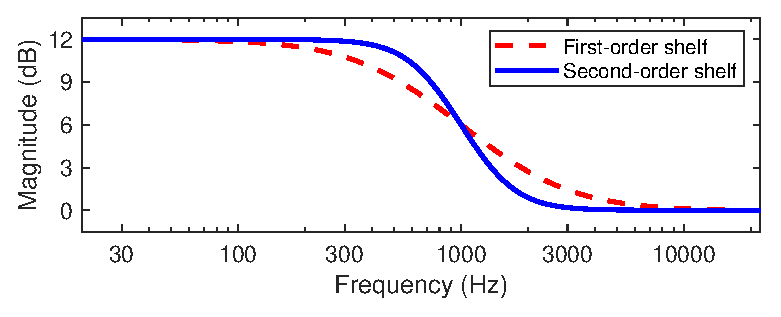
\includegraphics[width=82mm]{fig1_example.eps}
\caption{Figures using color must be understandable also in grayscale printing. It helps if both the line color and the line type are different for each curve.}
\label{fig:example_figure}
\end{figure}

For the final submission, photographic and bitmap images should be submitted as separate PNG files with a resolution of at least 300~dpi. JPEG files can be used, but are discouraged due to lossy compression. Line drawings can be submitted in EPS files. The figure number should be clearly indicated in the file name. The size of illustrations when formatted to the column size in the journal is usually \SI{82}{\milli\metre} (3.25~in) wide, although \SI{170}{\milli\meter} (6.75~in) wide can be used if required. 

Text labels on illustrations must be large enough so that the smallest letters are at least \SI{1.5}{\milli\metre} (1/16~in) high when the image is reduced to one of the above widths. If possible, text labels on all original illustrations should be scaled so that they will be the same size when reduced for reproduction in the journal. If not using \LaTeX, figure captions should either be inserted on a separate page of the main manuscript, following the references, or uploaded as a separate file. Captions should be concise, while ensuring the figure is comprehensible.

As an online journal, color figures are encouraged. However, it is still good practice to review all figures and associated captions and legends/keys to ensure that figures will be understandable if printed by readers in black and white.

\begin{figure*}
\centering
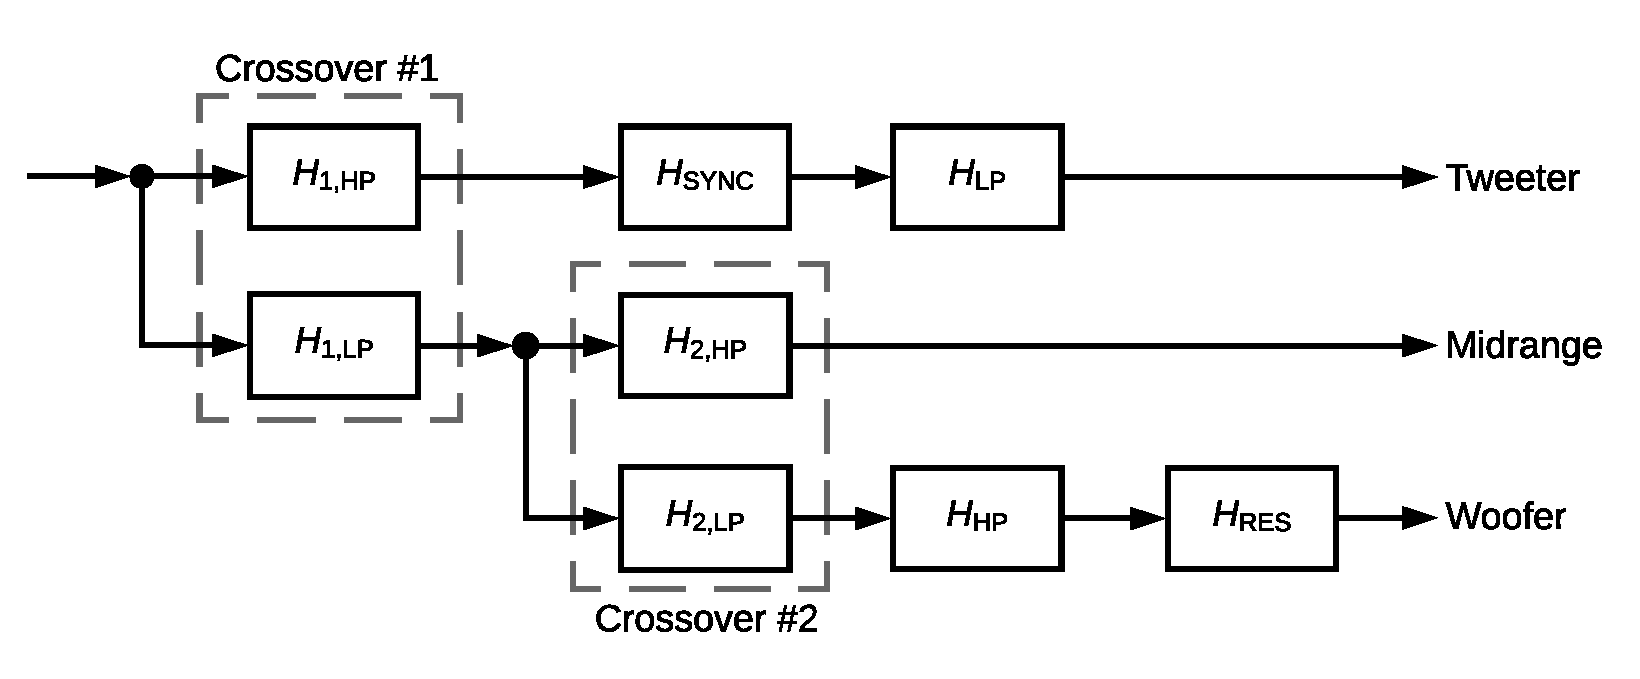
\includegraphics[trim=0cm 0.5cm 0cm 0.5cm, width=0.7\textwidth]{fig2_example.eps}
\caption{Example of a wide figure and caption extending over the two columns.}
\label{wide_figure}
\end{figure*}

\subsection{Tables}

\emph{JAES} articles often include tables, such as \cref{table:an_example_table}. They must be referred to and explained in text. 

%Table
\begin{table}[tb]
\tabcolsep8.1pt
\centering
\caption{Tables should have a brief caption. Highlighting the best result(s) is helpful to readers.}
\label{table:an_example_table}
{%
\begin{tabular}{@{}lllc@{}}\toprule
Excerpt No.& Genre & Spatial Mode & Correlation\\\colrule
 1 & Pop       & FB   & \textbf{94}\%\\
 2 & Classical & FB   & 33\%\\
 3 & Jazz      & FF   & 76\%\\
 4 & Arabian   & FF   & 41\%\\
 5 & GNE       & H220 & 45\%\\
 6 & GNE       & H45  & 93\%\\
 7 & MNK       & G416 & 74\%\\
 8 & MNK       & D413 & 72\%\\
 9 & MNK       & R420 & \textbf{94}\%\\
10 & MNK       & N516 & 91\%\\\botrule
\end{tabular}}
\begin{tabnote}
Note. This table contains several acronyms that should be defined in the paper, when they are first used (but not in the abstract).
\end{tabnote}
\end{table}

\subsection{Graphical Abstract}
Authors of a paper accepted for publication in \emph{JAES} are strongly encouraged to prepare a graphical abstract (GA) of the work performed. A GA is an image that summarizes the work in an eye-catching way, ideally summarizing the ideas of the paper. It appears alongside the text abstract in the online journal and AES E-Library. The GA may be a figure from the article or preferably one specially prepared for the purpose.\footnote{An example GA is available at: \url{https://www.aes.org/assets/base/img/content/journal/authors/guidelines/GraphicalAbstractExample4.png}.} A useful guide to preparing a GA can be found from Anna Clemens.\footnote{\url{www.annaclemens.com/blog/make-graphical-abstract-paper}.}

Any text in the image should be clear and readable, in a sans serif font such as Helvetica or Arial. No caption or additional descriptive text is expected. The image file for the GA needs to be a PNG (Portable Network Graphics) file and should be uploaded with the final version of your manuscript. It should be in portrait format, US Letter or A4 aspect ratio, with a minimum resolution of 600~pixels wide, and preferably in color.

\section{Reference Format and Digital Object Identifiers}\label{sec:refs}
References should be cited numerically in brackets in order of appearance in the text. References should be listed at the end of the text in order of appearance. In the reference list, please insert “and” between the last and second-to-last author name. Use a comma before “and” if there are more than two authors in the list. List up to five authors in a citation; references with six or more authors should have the first three authors listed, followed by ``et al.''  
In publication titles, all words should be capitalized except articles, conjunctions, and prepositions fewer than four letters, unless they are the first word of the title or follow a punctuation mark with the title, such as a colon. %In publication titles, the first letters of the first word and the main words are capitalized in the paper title, but not prepositions and articles (see examples below).

References to periodicals (journals) should include the authors’ names, title of article, periodical title abbreviation, volume, issue number, page numbers or article ID, year and month of publication, and the Digital Object Identifier (DOI) link, if available. The following are examples of the expected format of journal paper references \cite{a_journal_paper, a_journal_paper_with_many_authors, a_journal_paper_with_article_ID}.

Authors are expected to include DOIs for those references that have them. Manuscripts may be returned to authors to complete DOI referencing before a paper will be accepted for publication. Ideally, DOIs should be included for references when a paper is first submitted, avoiding additional delays. The journal is registered with CrossRef for the issuing of DOIs, and it is a condition of membership that \textit{JAES} provides outbound linking of references in its papers. This enables readers to find the papers to which your references refer easily. AES will also issue and register a DOI for your paper when it is published. Authors can look up individual DOIs using the free service provided by CrossRef\footnote{\url{http://www.crossref.org/guestquery/}.} or for multiple references in a list using the text query interface\footnote{\url{http://www.crossref.org/SimpleTextQuery/}.} (though you will have to validate your email address by setting up a free account).

Book references should contain the names of the authors, title of book, name and location of publisher, publication year, and edition (if other than first) \cite{a_book_ref, a_book_ref_2nd_edition}. A reference to a chapter published in an edited book should have the authors, the chapter name, the editors, the book title, the book series name, page numbers, the name and location of the publisher, publication year, and the edition number \cite{a_book_chapter}. 

For conference papers published in proceedings, please shorten the conference name. The conference acronym may optionally be shown in parentheses. The page numbers (if available, otherwise list page numbers as 1-$N$ with $N$ being the length of the manuscript), conference address (city, country/state), and year and month of the conference should also be shown, like in this example \cite{a_nonAESconference_paper}. The year of the conference is omitted from the conference name. For this reason, this reference example mentions the acronym ``ICASSP,'' not ``ICASSP-17'' \cite{a_nonAESconference_paper}. 
In a reference to an AES convention paper, the convention paper number can optionally be included, as in this example \cite{AES_convention_paper}. The paper's AES E-Library number link must be provided. References to AES convention papers should be replaced with the peer-reviewed journal publication citations if appropriately related journal papers have been published.

Presentations at conferences without published papers (e.g., abstract only) can be referenced as \cite{a_conference_presentation}. Please note that such references provide little scientific value, but can be used to note prior activity in the field. 

For a thesis reference, please include the author name, thesis title, type of thesis (Ph.D. thesis or M.Sc. thesis), the name and address (city, country/state) of the university, year, and month of publication. For example, this is a complete reference to a doctoral thesis \cite{a_PhD_thesis}, and this a reference to a Master's thesis \cite{an_MSc_thesis}. Links to online archives of thesis documents are also encouraged.

References to a patent should include the inventors’ names, patent title, specification of the patent (e.g., US or European patent) together with the patent number, and year and month of publication. The following is an example of the expected format of a patent reference in \emph{JAES} \cite{a_patent}. 

A web page reference should include the author, such as a company, the title of the web page, the web address (URL), and the date accessed. This is an example of a correctly referenced web site in \emph{JAES} \cite{a_web_page}. More examples of our current reference style may be viewed in recent issues of \emph{JAES}.

Preprint archive citations (e.g., arXiv) are suitable only for manuscripts currently under review elsewhere, when temporal priority must be established. Preprints are not peer-reviewed and have the same evidential validity as personal communications or blog postings. They represent the authors’ claims prior to independent verification. Citation of a preprint is therefore not acceptable as supporting evidence for scientific, technical, or factual assertions. It may only be used to acknowledge priority of discovery or to reference ongoing work. Preprints that have not been submitted for peer review, or that have been submitted and rejected, are not acceptable references for any purpose other than temporal priority. When a manuscript has been subsequently published, the published, peer-reviewed citation must be used as the official reference, not the preprint citation. An arXiv reference, for example, that is more than 1~year old can be assumed to be scientifically irrelevant. An arXiv download link may be used for file availability, equally for sites such as ResearchGate or University or national open science repositories (e.g., \url{https://hal.science/}), but the reference citation should be the actual reference. 

Some abbreviations are allowed in bibliographic references, such as ``Conf.'' for Conference. A listing of such abbreviations is given in \cref{table:abbrev} of \textsc{Appendix}~\ref{sec:abbreviations}.

\section{Author Information, Photographs, and Biographies}\label{sec:authophoto}
If authors are AES members, they should provide their status and AES member number on the author line. This is used for indexing in the AES library and other membership services. Members should indicate their current membership status as \emph{AES Student Member}, \emph{AES Associate Member}, \emph{AES Member}, or \emph{AES Fellow}.
The journal now supports ORCID. Authors are encouraged to include a link to their ORCID in the author line. 

For purely demographic statistics purposes, please not that the journal now asks authors and reviewers to report their gender. This in no way affects the peer-review process. Authors are here informed that this information is not communicated to reviewers. 

At the end of the manuscript, author photographs and biographies are required for each author for all Research Papers, Engineering Reports, and Review/Tutorial Papers. Each photograph should be a professional photo of the author’s face and the image must be able to be supplied as a separate, high-resolution graphic (PNG, EPS, or JPEG files with a resolution of at least 300~dpi). 

Author biographies should highlight each author’s education, places of employment, research visits, key research areas, professional memberships, and awards in 150~words or less. This section should appear after the references at the end of the manuscript file. Examples are given at the end of this template.

\section{Use of Artificial Intelligence and Large Language Models}\label{sec:AI-LLM} 

Authors who use AI technologies, including LLMs or other generative tools (for text, image, or data creation), in the preparation of a manuscript must adhere to the following principles:

\begin{itemize}
  \item Appropriate use:
  Use of AI or LLM tools for limited editorial tasks such as spelling, grammar, or formatting corrections is permitted and does not require disclosure. However, substantive drafting or generation of text, data, or figures must be fully disclosed and justified.
  Unless clearly described as part of the research method, AI-generated content cannot replace the authors’ core intellectual contribution.
  
  \item Authorship and responsibility:
  AI or LLM tools cannot be listed as authors. All listed authors must meet the journal’s authorship criteria and accept full responsibility for the integrity of the work.
  
  \item Disclosure and transparency:
  At submission, authors must disclose any use of AI, LLM, or generative-tool assistance in any part of the manuscript (e.g., text drafting, data generation, figure creation, or editing). The disclosure, in a section-relevant footnote or in the acknowledgments, should include the tool name, version, model, date of use, manufacturer (if applicable), and a brief description of how the tool was used.

  \item Verification and accountability:
  Human authors must critically review, verify, and take full responsibility for all content, including text, figures, data, tables, references, and interpretations. AI-generated or AI-edited material must meet the same standards of originality, accuracy, ethics (including avoidance of plagiarism and data fabrication), and attribution as any other content.

  \item Citation and attribution:
  AI tools must not be cited as authors or treated as unreferenced original content.   Any material generated via AI or LLM must be clearly attributed or acknowledged, and its provenance must be traceable.

  \item Ethical compliance:
  Authors must not input confidential, personal, or proprietary data into AI or LLM systems.
  Use of such tools must not compromise confidentiality, peer-review ethics, or data integrity.
\end{itemize}

\section{General Requirements}\label{sec:general}
All material published by the AES, regardless of the type, shall conform to the following requirements unless specifically exempted by Publications Policy or by the Editor.

\begin{itemize}
    \item Style: The technical content should be accurate; the writing should use good grammar and be easy to understand by those versed in the art. Abbreviations, units, and definitions of quantities should conform to the AES editorial style.
    
    \item Good taste: Good taste is a necessity. No derogatory mention of other engineering work, engineers, or organizations shall be made. Constructive technical criticism, which makes a suggestion(s) for improvement(s) that would remove the objection, is not derogatory if the technical basis is well developed and accurate. The Editorial Office should ask reviewers to judge carefully the substance of such criticism. Specifically, the initiation of controversy should be minimized by a careful checking of the critical judgments. Controversy for its own sake should be discouraged.
    
    \item Commercialism: A manuscript that is based on a commercial product should be reviewed extremely carefully to determine the real scientific content (including Engineering Reports). If a manuscript has no other merit than as a description of the product, it is not acceptable. This requirement is especially important in articles that provide technical results without an adequate description of a device’s operation.
    
    \item Original unpublished work: Manuscripts should describe original work unpublished elsewhere or that is not being considered for publication elsewhere. The Editor may also reject manuscripts that are original but too similar to other published work. Publications of AES conference/convention papers, or of other meetings at the discretion of the Editor, may be further reviewed and republished in \emph{JAES}, but only after they have been revised and extended. A typical guideline is at least \SI{30}{\percent} new material relative to a prior published conference manuscript.
    
    \item Trademarks: Trademarks are generally inappropriate because they serve a commercial purpose, not an engineering purpose. (a)~Trademark symbols are not permitted. (b)~Trademark names in titles and abstracts should be replaced by generic descriptions where possible. If trademarked names are retained in titles and abstracts, they will not be acknowledged as such. (c)~The first time a trademarked name appears in the body text, it may be footnoted. The footnote will state that it is registered and the name of the owner.
\end{itemize}

\section{Conclusion}\label{sec:conc}
The manuscript submitted to \emph{JAES} should end with a section entitled ``Conclusion''. The Conclusion should briefly review the main points of the paper and its relation to the state of the art. However, do not replicate the abstract. All results mentioned in the Conclusion must be deducted from the other parts of the paper. Do not introduce new results in the Conclusion. This section may also speculate on applications and extensions of the results (future work). Many readers browsing technical papers only read the abstract and the Conclusion.

\section{Copyright}\label{sec:Copyright}

For questions related to copyright, reproduction, republication, reuse, and other related issues, authors are directed to \url{https://aes.org/publications/open-access-publications-policy/} for the latest information. 

\section{Acknowledgment}
This  work  has  been  funded  in  part  by  the Agence nationale de la recherche (ANR project no.~123456). This template version was edited by Kurt James Werner, Vesa V\"alim\"aki, and Brian F.G. Katz. 

% - If you are using bibTex for references, you need these lines: 
\bibliography{jaes.bib}
\bibliographystyle{jaes.bst}

% NOTE:
% - in case you are not using bibTex you have to manually edit the bibliograpy as below.
%%%%%%%%%%%%%%%%%%%%%%%%%%%%%%%%%%
% \begin{thebibliography}{10}
% \newcommand{\enquote}[1]{``#1''}
% \providecommand{\url}[1]{\texttt{#1}}
% \providecommand{\urlprefix}{URL }
% \expandafter\ifx\csname urlstyle\endcsname\relax
%   \providecommand{\doi}[1]{[Online]. Available: \discretionary{}{}{}#1}\else
%   \providecommand{\doi}{doi:\discretionary{}{}{}\begingroup \urlstyle{rm}\Url}\fi

% \bibitem{a_journal_paper}
% Y.~Li, J.~Cai, Q.~Dong, L.~Wu, and Q.~Chen, \enquote{Psychophysiological Responses of Young People to Soundscapes in Actual Rural and City Environments,} \emph{J. Audio Eng. Soc.}, vol.~68, no.~11, pp. 910--925 (2020 Dec.), \doi{10.17743/jaes.2020.0060}.

% \bibitem{a_journal_paper_with_many_authors}
% T.~Fujioka, C.~Freigang, K.~Honjo, J.~J. Chen, J.~L. Chen, S.~E. Black, \emph{et~al.}, \enquote{Central Auditory Processing in Adults with Chronic Stroke Without Hearing Loss: A Magnetoencephalography Study,} \emph{Clin. Neurophysiol.}, vol. 131, no.~5, pp. 1102--1118 (2020 May), \doi{10.1016/j.clinph.2020.01.014}.

% \bibitem{a_journal_paper_with_article_ID}
% S.~Ntalampiras, I.~Potamitis, and N.~Fakotakis, \enquote{Exploiting Temporal Feature Integration for Generalized Sound Recognition,} \emph{EURASIP J. Adv. Signal Process.}, vol. 2009, no.~1, paper 807162 (2009 Dec.), \doi{10.1155/2009/807162}.

% \bibitem{a_book_ref}
% V.~Pulkki and M.~Karjalainen, \emph{Communication Acoustics: An Introduction to Speech, Audio and Psychoacoustics} (Wiley, Chichester, UK, 2015).

% \bibitem{a_book_ref_2nd_edition}
% D.~Oram, \emph{An Individual Note of Music, Sound and Electronics}, 2nd ed. (Anomie Academic, Swindon, UK, 2016).

% \bibitem{a_book_chapter}
% V.~V\"alim\"aki, S.~Bilbao, J.~O. Smith, J.~S. Abel, J.~Pakarinen, and D.~Berners, \enquote{Virtual Analog Effects,} in U.~Z\"olzer (Ed.), \emph{DAFX---Digital Audio Effects}, pp. 473--522 (John Wiley \& Sons, Chichester, UK, 2011), 2nd ed.

% \bibitem{a_nonAESconference_paper}
% S.~J. Schlecht and E.~A. Habets, \enquote{Accurate Reverberation Time Control in Feedback Delay Networks,} in Proceedings of the \emph{International Conference on Digital Audio Effects (DAFx)}, pp. 337--344 (2017 Sep.).

% \bibitem{AES_convention_paper}
% M.~Gospodarek, A.~Genovese, D.~Dembeck, C.~Brenner, A.~Roginska, and K.~Perlin, \enquote{Sound Design and Reproduction Techniques for Co-Located Narrative VR Experiences,} in Proc. of the \emph{147th Convention of the Audio Engineering Society} (2019 Oct.),  \href{https://aes2.org/publications/elibrary-page/?id=20660}{AES e-library 20660}, paper 10287.

% \bibitem{a_conference_presentation}
% A.~Andreopoulou and B.~F.~G. Katz, \enquote{Identifying a perceptually relevant estimation method of the Inter-aural Time Delay,} presented at the \emph{Meeting of Acoustical Society of America}, vol. 141, p. 3635 (Boston) (2017).

% \bibitem{a_PhD_thesis}
% P.~D. L.~G. Pestana, \emph{Automatic Mixing Systems Using Adaptive Digital Audio Effects}, Ph.D. thesis, Universidade Cat\'olica Portuguesa, Porto, Portugal (2013 Feb.), \urlprefix\url{http://hdl.handle.net/10400.14/10887}.

% \bibitem{an_MSc_thesis}
% J.~Holm, \emph{Applying the Finite Element Method for Modelling Loudspeaker Waveguide Directivity}, Master's thesis, Aalto University, Espoo, Finland (2010 May), \urlprefix\url{http://lib.tkk.fi/Dipl/2010/urn100200.pdf}.

% \bibitem{a_patent}
% P.~G. Craven and M.~A. Gerzon, \enquote{Coincident Microphone Simulation Covering Three Dimensional Space and Yielding Various Directional Outputs,} {US} Patent 4,042,779 (1977 Aug.).

% \bibitem{a_web_page}
% {Audio Engineering Society}, \enquote{Journal Author Guidelines,} \url{https://aes2.org/publications/journal-of-the-audio-engineering-society/journal-author-guidelines/} (accessed Nov. 21, 2025).

% \end{thebibliography}

%%%%%%%%%%%%%%%%%%%%%%%%%%%%%%%%%%

%Appendix
\appendix

\section{\MakeUppercase{Appendix usage}}
One or more appendixes can appear after the references. Each appendix must have its own title. An appendix can present, for example, a mathematical derivation, pseudo-code, or other additional data that is unsuitable to show in the body of the article. Tables, figures, and equations included in appendixes are numbered based on where they left off in the text (they do not restart with ``1'' or have labels like ``Figure A.2''). Appendix tables, figures, and equation labels match and follow from those of main article tables, figures, and equations, such as \cref{fig:AESlogo}.

\begin{figure}[!ht]
\centering

\includegraphics[alt={JAES logo},trim=0cm 0.cm 0cm 0.cm, width=.85\columnwidth]{JAESlogo.png}
\caption{Example of a figure in an appendix.}
\label{fig:AESlogo}
\end{figure}

\section{\MakeUppercase{Acronyms in titles}}\label{sec:ackronyms}

\Cref{table:acronyms} lists commonly accepted and unambiguous acronyms which are sufficiently well-known that they can be used within journal titles. Please contact the journal's Editor in Chief if you would like to propose an additional term. 

\begin{table}[!ht]
    \caption{JAES acronyms approved for use in article titles.}\label{table:acronyms}
    \begin{tabular}{@{}ll@{}}
    \toprule
        Acronym & Definition \\
    \colrule
        3-D & Three-dimensional \\
        3D & Three-dimensional \\
        AES & Audio Engineering Society \\
        AM & Amplitude Modulation \\
        DFT & Discrete Fourier Transform \\
        DNN & Deep Neural Network \\
        DSP & Digital Signal Processing \\
        FFT & Fast Fourier Transform \\
        FM & Frequency Modulation \\
        HRTF & Head-Related Transfer Function \\
        MIDI & Musical Instrument Digital Interface communication protocol \\
        MPEG & Moving Picture Experts Group \\
        SNR & Signal-to-Noise Ratio \\
        SPL & Sound Pressure Level \\
        STFT & Short-Time Fourier Transform \\
    \botrule
    \end{tabular}
\end{table}

\section{\MakeUppercase{Abbreviations in bibliography}}\label{sec:abbreviations}

\Cref{table:abbrev} lists commonly accepted and unambiguous acronyms which are sufficiently well-known that they can be used within journal titles. Please contact the journal's Editor in Chief if you would like to propose an additional term. 

\begin{table}[!ht]
    \caption{JAES abbreviations approved for use in bibliography.}\label{table:abbrev}
    \begin{tabular}{@{}ll@{}}
    \toprule
        Abbreviation & Definition \\
    \colrule
        Colloq. & Colloquium \\
        Conf. & Conference \\
        Cong. & Congress \\
        Conv. & Convention \\
        Intl. & International \\
        J. & Journal \\
        Proc. & Proceedings \\
        Q. & Quarterly \\
        Symp. & Symposium \\
    \botrule
    \end{tabular}
\end{table}

\clearpage % include as there are formatting conflicts with the end of the manuscript in 2-column format and the Biography section. 

%Biography
 \biography{Jean Dupont}{headshot1.jpg}{Jean Dupont is a professor of audio technology at XYZ University, Paris, France. He received his M.Sc. and Ph.D.~degrees from Sorbonne University in 1992 and in 1995, respectively. In 1996, he was a postdoctoral research fellow at the University of Westminster, London, UK. In 2001--2002, he was a professor of signal processing at the Pori School of Technology and Economics, Tampere University of Technology, Pori, Finland. In 2008--2009, he was a visiting scholar at the Center for Computer Research in Music and Acoustics (CCRMA), Stanford University, Stanford, CA. His research interests include musical signal processing, digital filter design, and acoustics of musical instruments. Prof. Dupont is a senior member of the IEEE and is a member of the Société Française d'Acoustique. He was the Chair of the 11th International Conference on Digital Audio Effects (DAFx), which was held in Espoo, Finland, in 2008.}
 
 \biography{Jane Doe}{headshot2.jpg}{Jane Doe is a senior scientist at Audio Technology Company, Los Angeles, CA, where her research interests include audio and music applications of signal and array processing, parameter estimation, and acoustics. She holds Ph.D.~and M.S.~degrees from Stanford University, and an S.B.~from MIT, all in electrical engineering. Dr.~Doe was a researcher at NASA/Ames Research Center, exploring topics in room acoustics and spatial hearing on a grant through the San Jose State University Foundation. She was also chief scientist of Crystal River Engineering, Inc., where she developed their positional audio technology, and a lecturer in the Department of Electrical Engineering at Yale University. Dr.~Doe is a Fellow of the Audio Engineering Society.}

\end{document}
